\documentclass{article}
\usepackage[utf8]{inputenc}
\usepackage[T1]{fontenc}
\usepackage[utf8]{inputenc}
\usepackage[norsk]{babel}
\usepackage{amsmath}
\usepackage{hyperref}
\usepackage{enumerate}
\usepackage{graphicx}
\usepackage{listings}
\usepackage{color}
\usepackage{gensymb}
\definecolor{codegreen}{rgb}{0,0.6,0}
\definecolor{codegray}{rgb}{0.5,0.5,0.5}
\definecolor{codepurple}{rgb}{0.58,0,0.82}
\definecolor{backcolour}{rgb}{0.95,0.95,0.92}
\setlength{\parindent}{0pt}
\lstdefinestyle{mystyle}{
    backgroundcolor=\color{backcolour},
    commentstyle=\color{codegreen},
    keywordstyle=\color{magenta},
    numberstyle=\tiny\color{codegray},
    stringstyle=\color{codepurple},
    basicstyle=\footnotesize,
    breakatwhitespace=false,
    breaklines=true,
    captionpos=b,
    keepspaces=true,
    numbers=left,
    numbersep=5pt,
    showspaces=false,
    showstringspaces=false,
    showtabs=false,
tabsize=2}
\lstset{style=mystyle}

\title{Oblig1 INF2270}
\author{mathiaki}
\date{February 2017}

\begin{document}

\maketitle

\newpage
\tableofcontents
\newpage

\section{Texture discription}
First, when i describe the different textures, i will index the different images in the following way: (the same is true for the program)\\
\begin{verbatim}
 img0        img1      img0     img1
|---|---| |---|---| |-------| |-------|
| 0 | 1 | | 4 | 5 | |       | |       |
|---|---| |---|---| |   8   | |   9   |
| 2 | 3 | | 6 | 7 | |       | |       |
|---|---| |---|---| |-------| |-------|

\end{verbatim}

This means i will start in the top left corner of mosaic1 and and in the bottom right corner of mosaic2. In the program 8 and 9 is reserved for the whole mosaic1 and mosaic2 respectivly. 

\subsection{Texture 0}
\textbf{disc of texture}
\textbf{disc of texture}
\textbf{disc of texture}
\textbf{disc of texture}
\textbf{disc of texture}
\textbf{disc of texture}
\begin{figure}[h!]
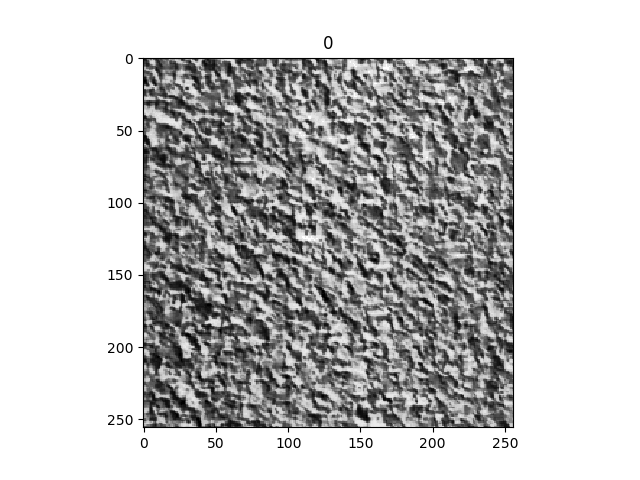
\includegraphics[scale=0.5]{0.png}
\end{figure}

\newpage
\subsection{Texture 1}
\textbf{disc of texture}
\textbf{disc of texture}
\textbf{disc of texture}
\textbf{disc of texture}
\textbf{disc of texture}
\textbf{disc of texture}
\begin{figure}[h!]
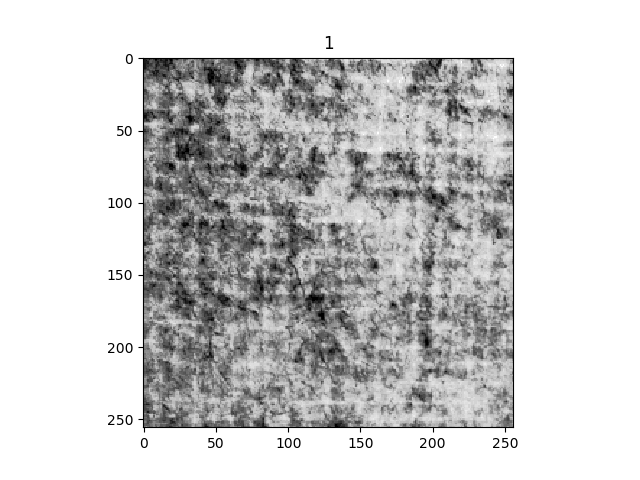
\includegraphics[scale=0.5]{1.png}
\end{figure}


\subsection{Texture 2}
\textbf{disc of texture}
\textbf{disc of texture}
\textbf{disc of texture}
\textbf{disc of texture}
\textbf{disc of texture}
\textbf{disc of texture}
\begin{figure}[h!]
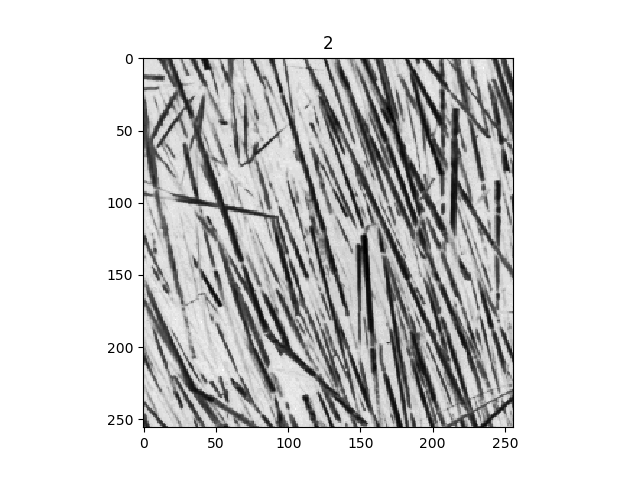
\includegraphics[scale=0.5]{2.png}
\end{figure}
\newpage

\subsection{Texture 3}
\textbf{disc of texture}
\textbf{disc of texture}
\textbf{disc of texture}
\textbf{disc of texture}
\textbf{disc of texture}
\textbf{disc of texture}
\begin{figure}[h!]
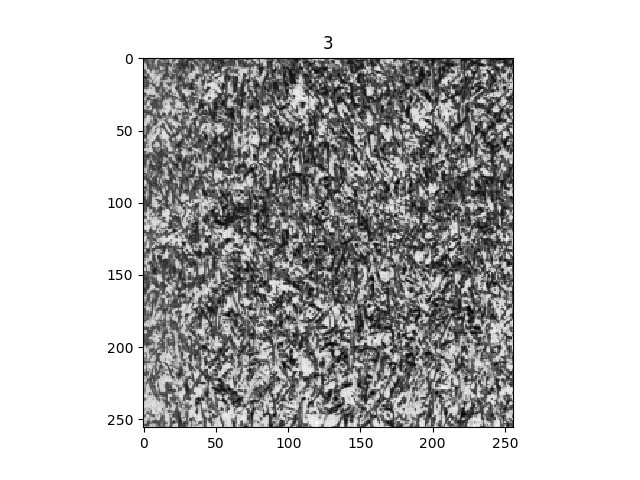
\includegraphics[scale=0.5]{3.png}
\end{figure}


\subsection{Texture 4}
\textbf{disc of texture}
\textbf{disc of texture}
\textbf{disc of texture}
\textbf{disc of texture}
\textbf{disc of texture}
\textbf{disc of texture}
\begin{figure}[h!]
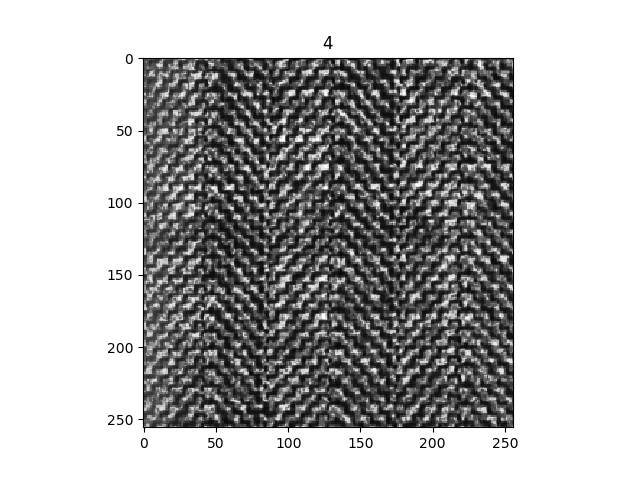
\includegraphics[scale=0.5]{4.png}
\end{figure}
\newpage

\subsection{Texture 5}
\textbf{disc of texture}
\textbf{disc of texture}
\textbf{disc of texture}
\textbf{disc of texture}
\textbf{disc of texture}
\textbf{disc of texture}
\begin{figure}[h!]
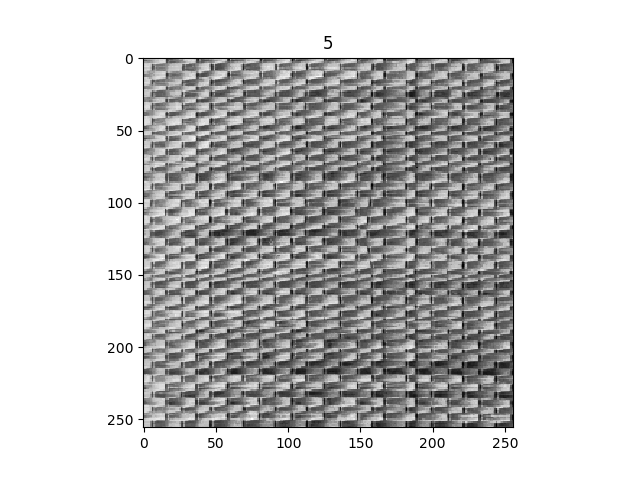
\includegraphics[scale=0.5]{5.png}
\end{figure}




\end{document}\\

